\section{Implementation and Performance Evaluation}
\label{sec:implementationEvalution}
%�����ϸ�ڿ��ǣ�Ӧ�÷�������
%\vspace{-1mm}
The evaluation platform is a Lenovo ThinkCentre M8400t PC with an Intel Core i7-2600 CPU and 2GB RAM.
 This CPU has $4$ cores and each core has a $32$KB L1 data cache. The operating system is 32-bit Linux with kernel version 3.6.2.


\subsection{Implementation}

%\vspace{-1mm}
% AES  mbed TLS-2.4.2
%In this section,
We apply the {\scshape{Warm+Delay}} scheme to AES-128. %to validate the security and evaluate the performance.
The implementation of AES employs the OpenSSL-1.0.2c~\cite{openssl} with a 2K lookup table.
As we aim to provide the optimized performance while eliminating remote cache timing side
channels, efficient {\scshape{GetTime()}}, {\scshape{Warm()}} and {\scshape{Delay()}}
  are finished;
and the constant parameters (TWOCM and WET) are determined properly.
 Next, we show the implementation details about the {\scshape{Warm+Delay}} scheme.

\noindent\textbf{AES implementation.}
Even when all lookup tables are in the L1 cache, the encryption time still has some variations(Figure~\ref{fig:fullwarmese-diffinput}). There are two main reasons. One is the cache bank conflict. Each cache bank can only serve one request at a time. So, multiple accesses to the same cache bank are slower than to different banks. The other is that the load from L1 cache takes slightly more time if it involves the same set of cache lines as a recent store.
These variations can be exploited by attackers~\cite{Canteaut2006Understanding,Bernstein2005Cache}.

For the cache bank conflict,
 we first close the Hyper-Threading of the system to ensure the protected process itself not to produce concurrent access to the cache.
  Then in the remote environment, the attackers cannot run the attack process on the target,
   so the attack in \cite{} can not be launched.
We avoid the second cause by exploiting the stack switch technique~\cite{guan2014copker}. The aligned consecutive lookup table distributes in 32 cache sets due to the cache mapping rule while the total number of cache sets is 64 on our platform.
We declare a 2KB global array as the stack, with which we can easily control the address.
The starting address of the array is made next to the lookup table module 4096, and this make the intermediate variables of AES execution use the remaining cache sets compared with the lookup table.
In this case, the distribution of AES encryption for $2^{30}$ random plaintexts is shown in Figure~\ref{fig:fullwarmbest}.
Served as a contrast, the Figure~\ref{fig:fullwarmworst} shows the distribution that the first address of the array is the same as the lookup table module 4096.
\begin{figure}[t]
\centering
%\subfigure[different inputs]{
%\centering
%\begin{minipage}[b]{0.6\textwidth}
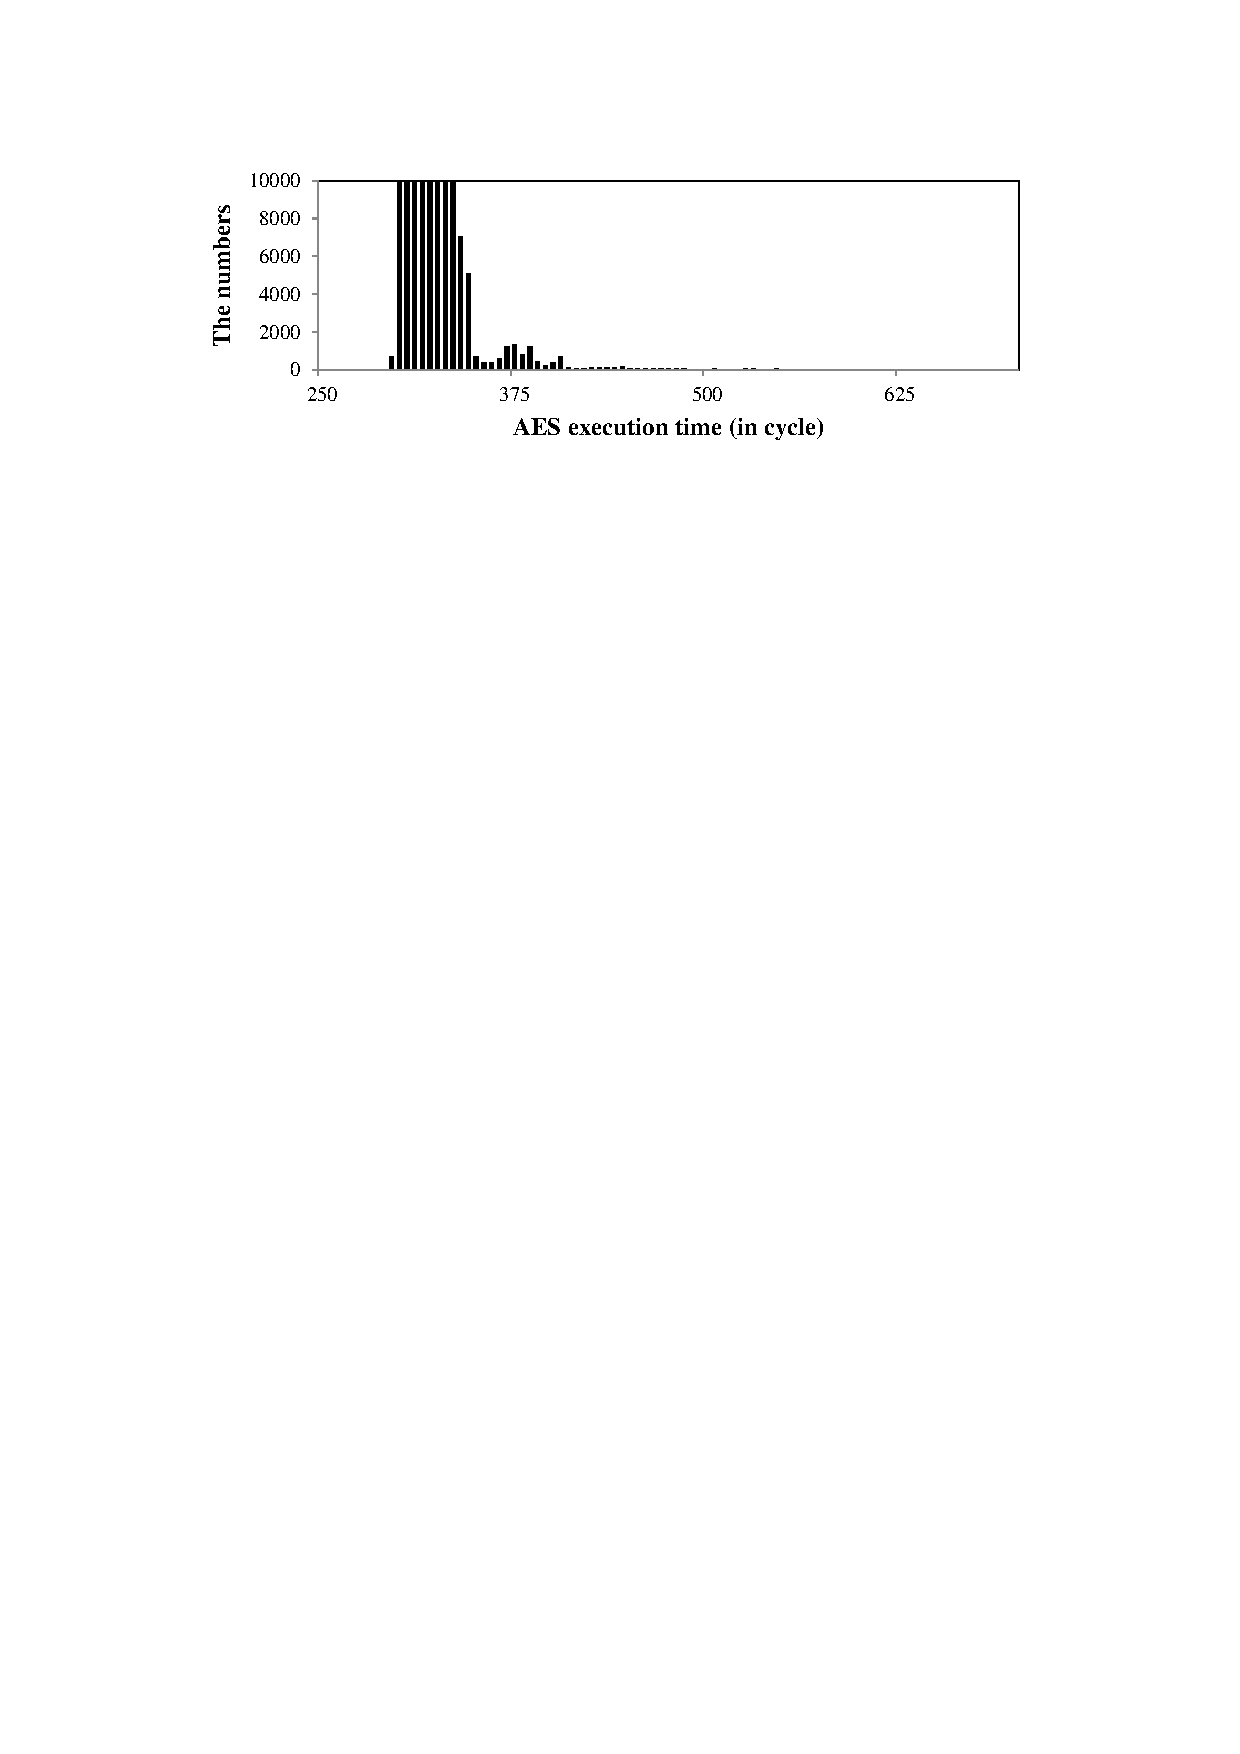
\includegraphics[width=0.7\textwidth]{pic/TWOCM_allwarm.pdf}

%\end{minipage}
%}
%\subfigure[same inputs]{
%\centering
%\begin{minipage}[b]{0.6\textwidth}
%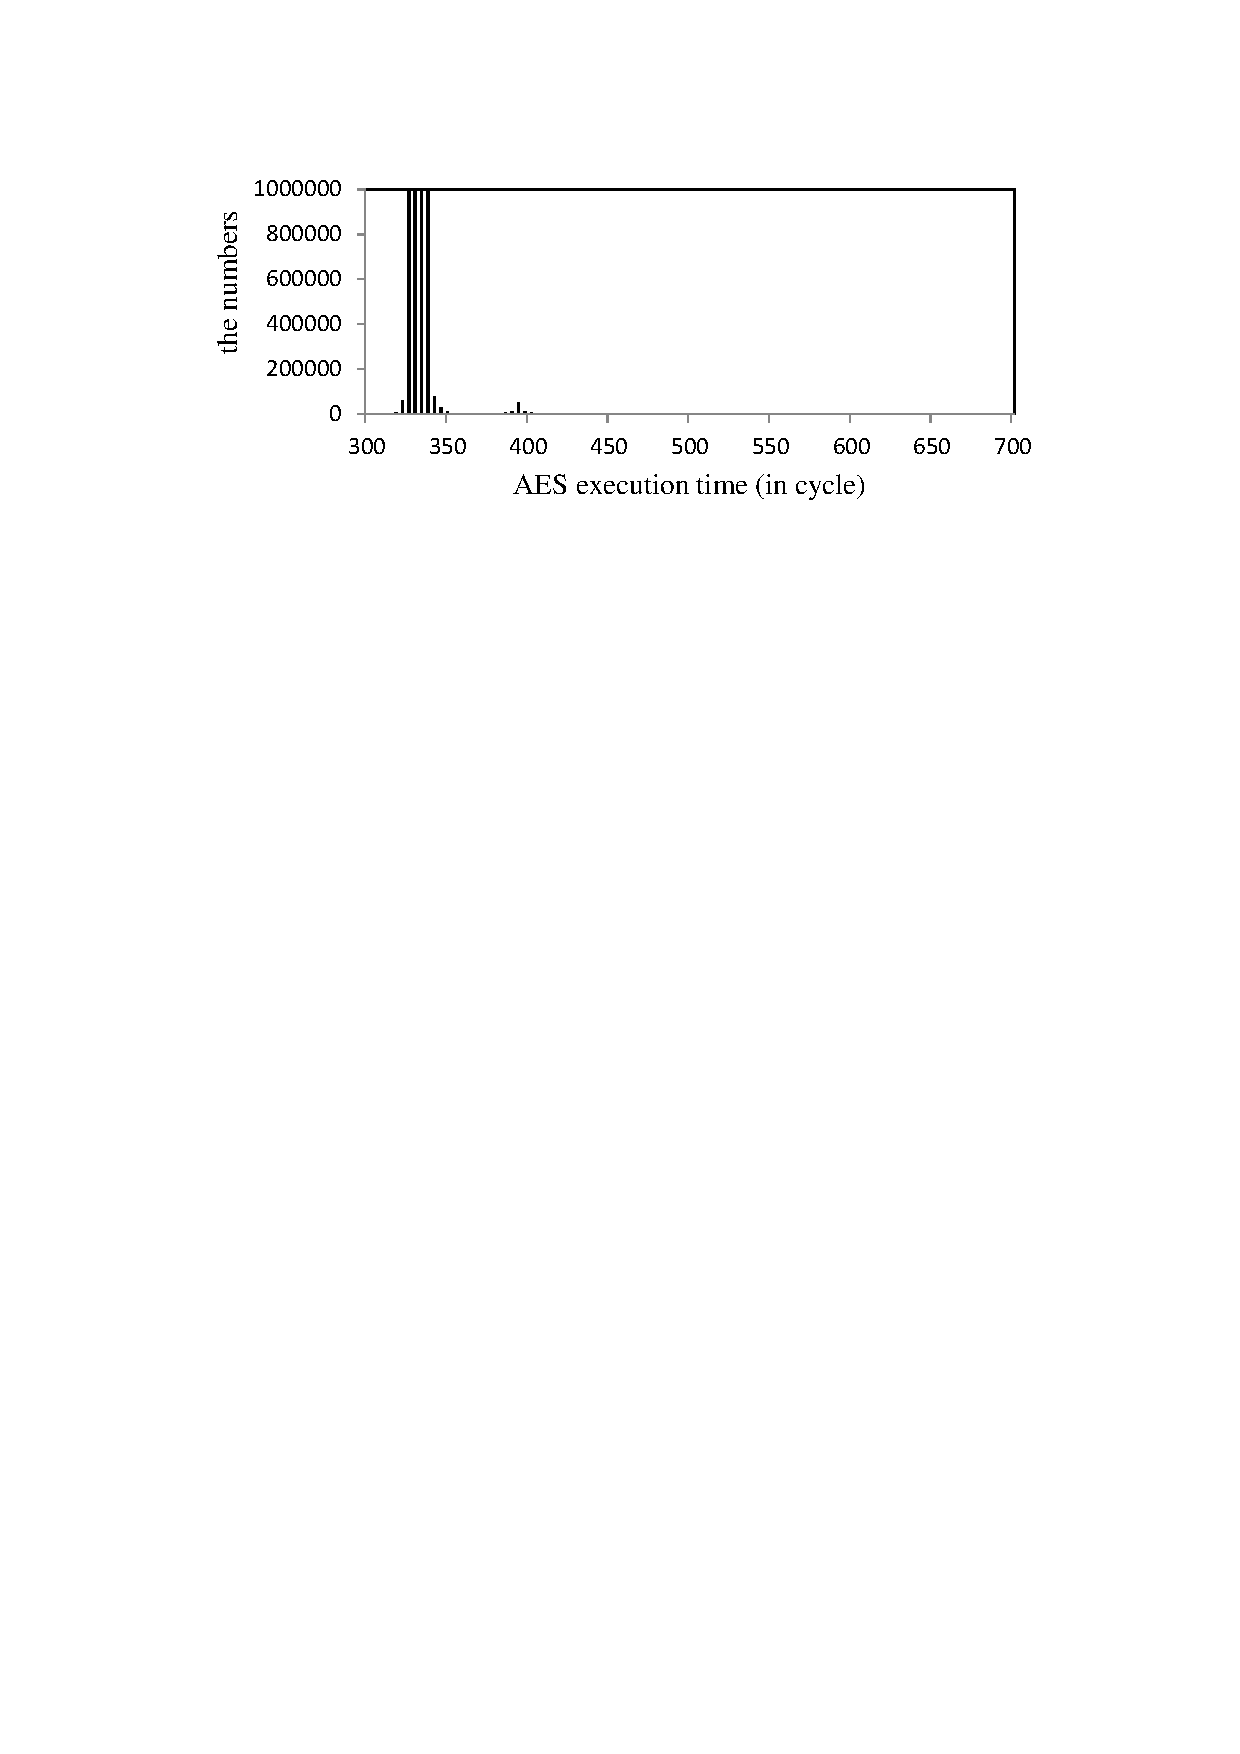
\includegraphics[width=1\textwidth]{pic/fullwarmsin.pdf}
%\label{fig:fullwarmese-sameinput}
%\end{minipage}
%}
 \caption{The distribution of AES encryption time in full warm condition.} \label{fig:fullwarmese-diffinput}
\end{figure}

\begin{figure}[t]
\centering
\subfigure[the worst case]{
\centering
\begin{minipage}[b]{0.6\textwidth}
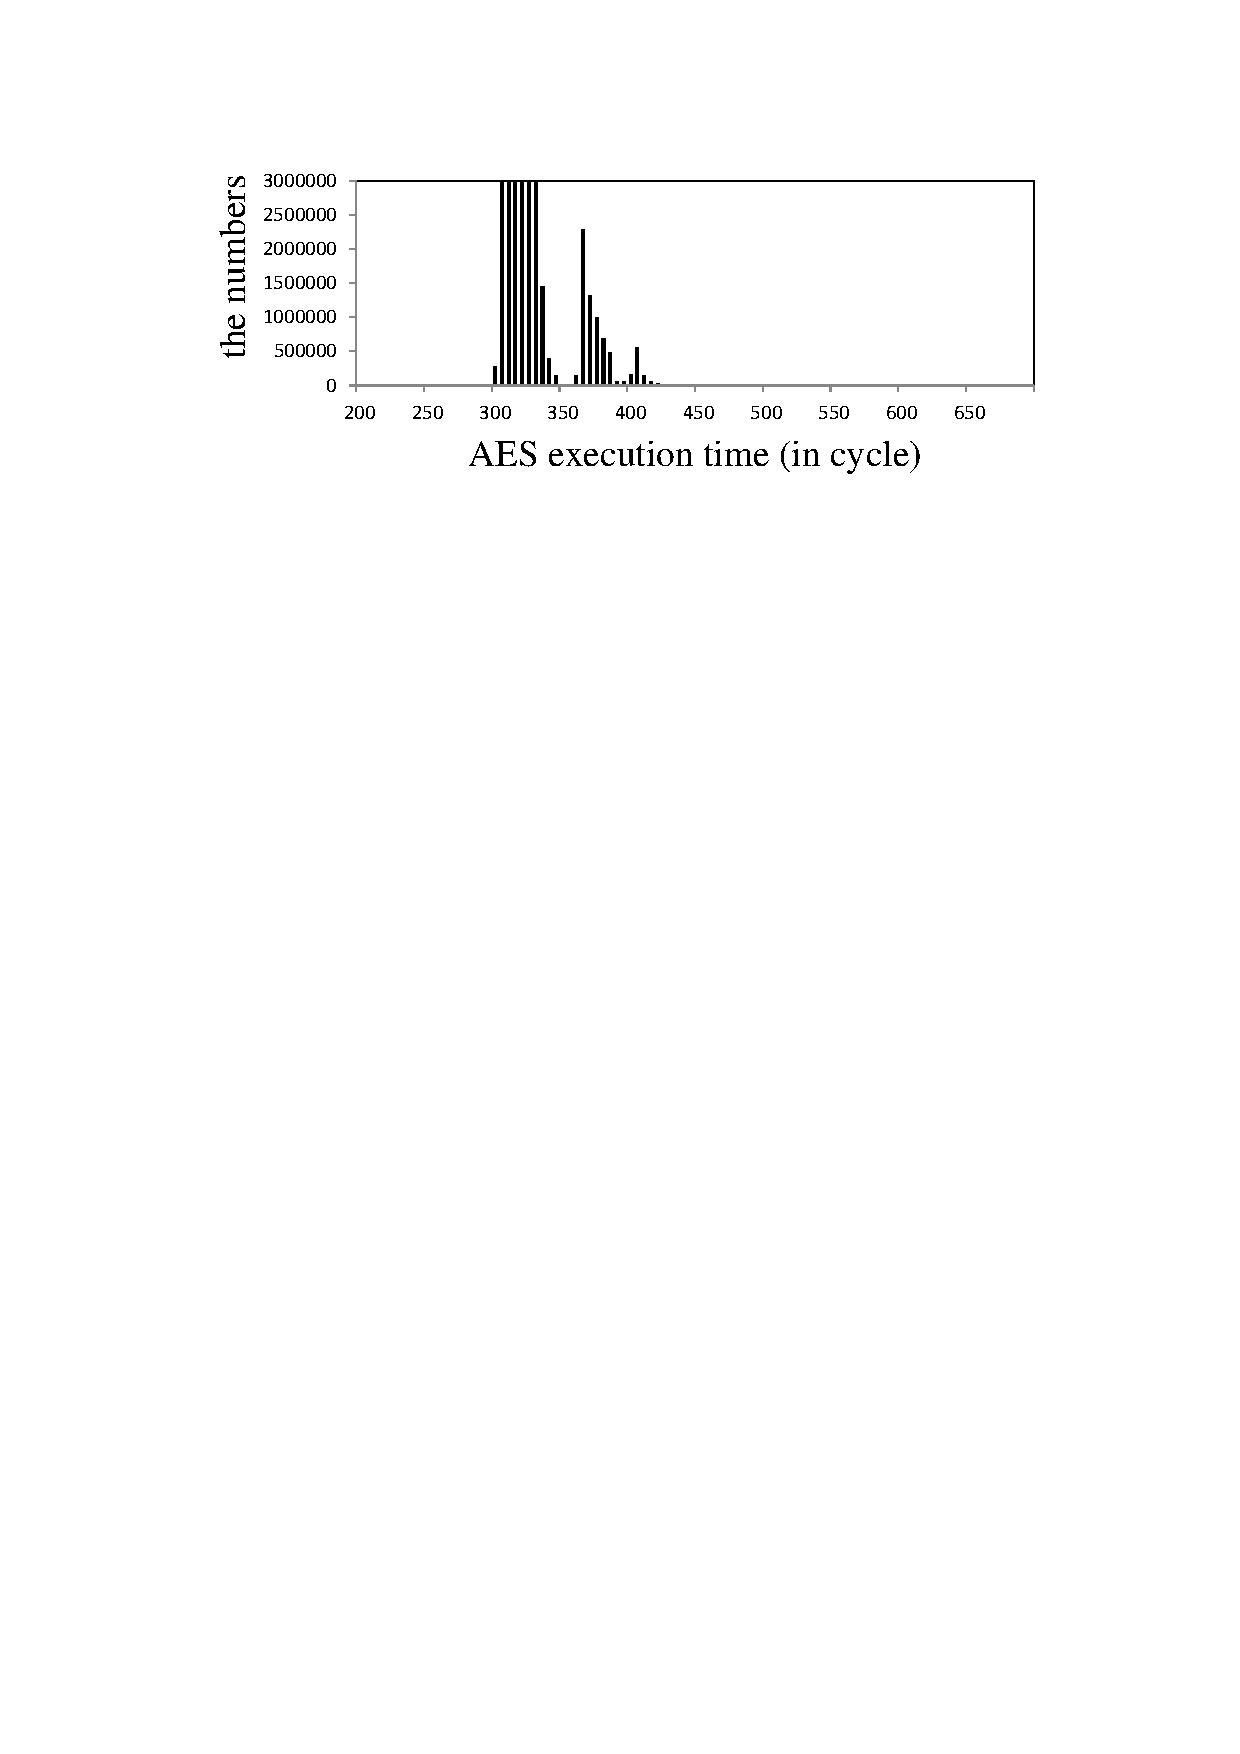
\includegraphics[width=1\textwidth]{pic/fwopensslworst.pdf}
\label{fig:fullwarmworst}
\end{minipage}
}
\subfigure[the best case]{
\centering
\begin{minipage}[b]{0.6\textwidth}
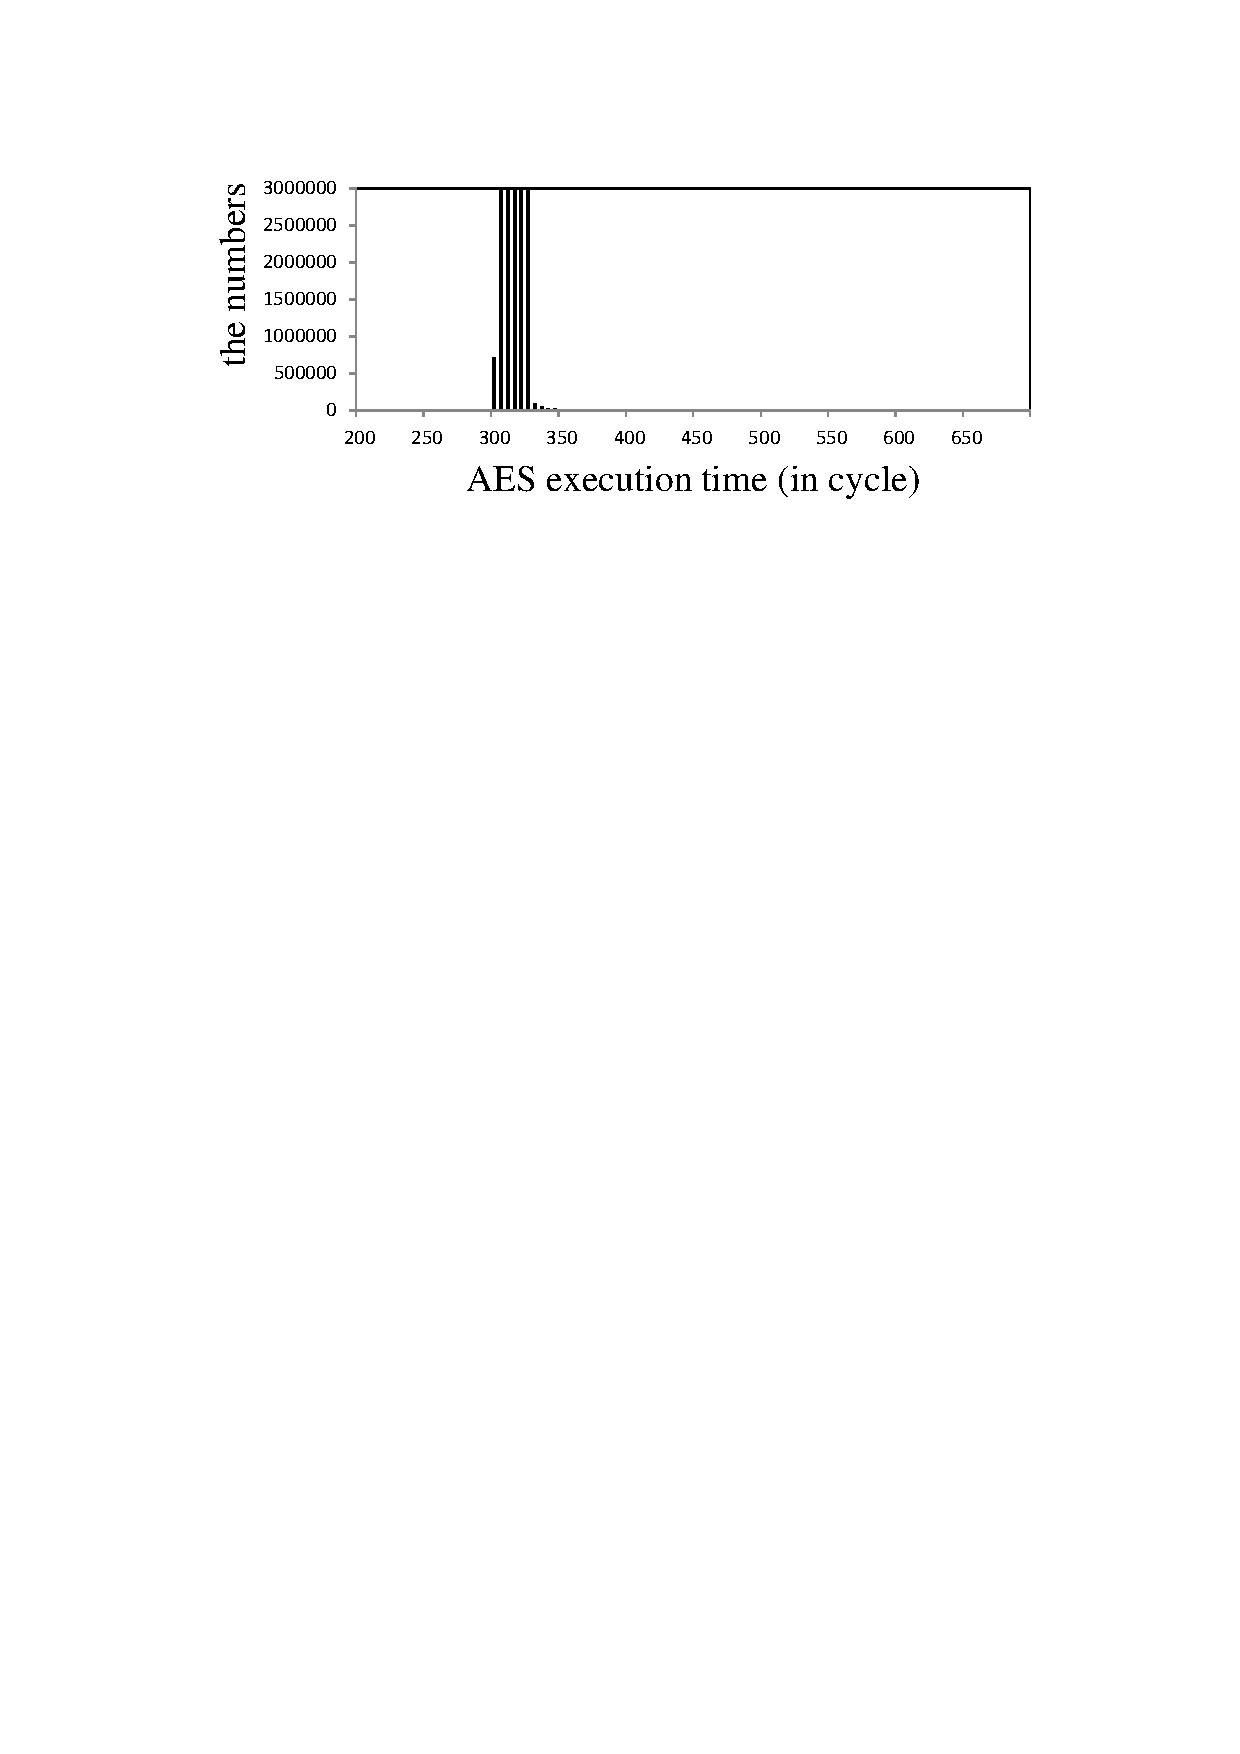
\includegraphics[width=1\textwidth]{pic/fwopensslbest.pdf}
\label{fig:fullwarmbest}
\end{minipage}
}
 \caption{The distribution of AES encryption time with 2KB lookup table in full warm condition.}
\end{figure}

%In our environment, for each of $2^{30}$ random plaintexts, we perform the encryption after loading  all the lookup tables into cache. Figure~\ref{fig:fullwarmese-diffinput} describes the distribution of encrypting time.

\begin{figure}[t]
  \centering
  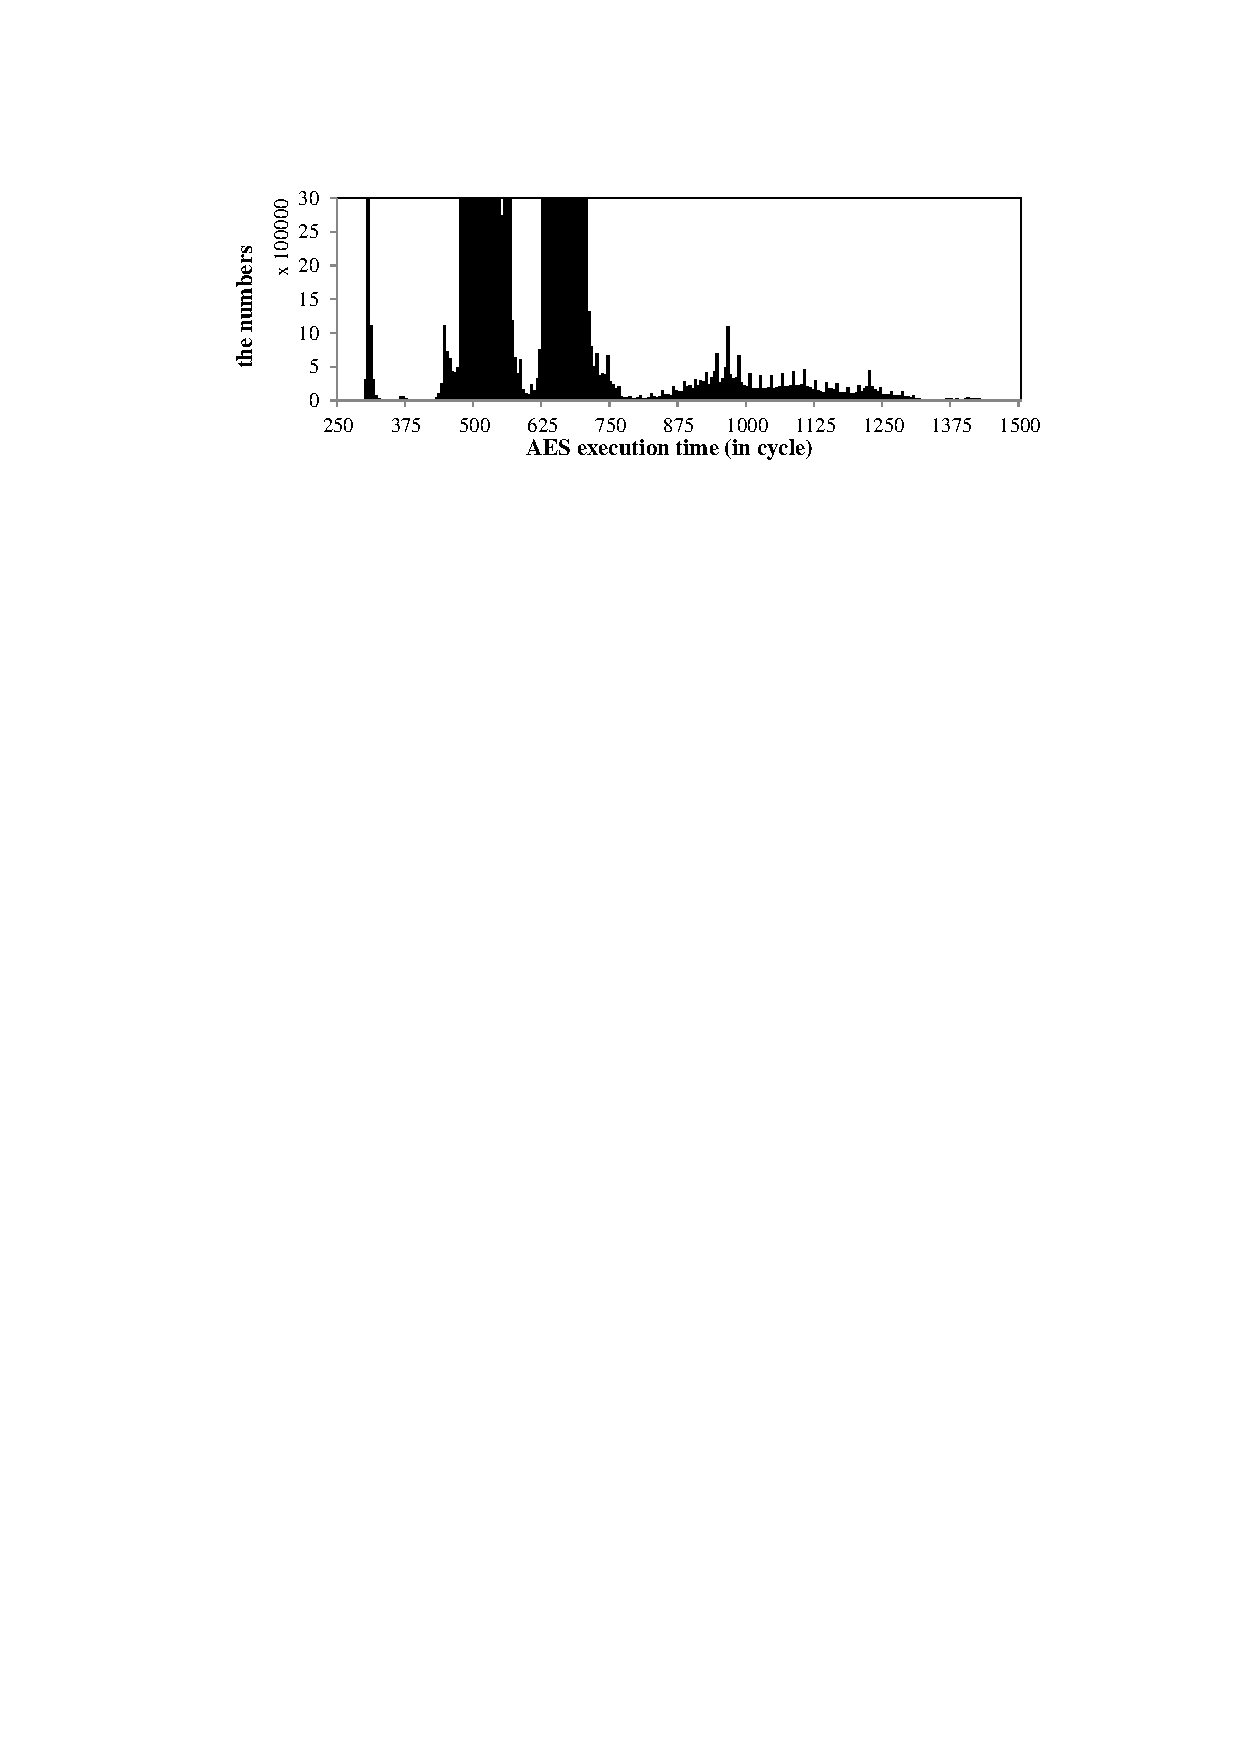
\includegraphics[width=0.55\textwidth]{pic/TWOCM_onenotin.pdf}\\
  \caption{The distribution of AES execution time only  not warm one cache line.}\label{fig:twocm}
\end{figure}

\noindent\textbf{TWOCM.}
TWOCM is larger than the minimum AES execution time (no cache miss occurs), which avoids the unnecessary {\scshape{Warm()}} and {\scshape{Delay()}} operations;
and less than the AES execution that only one cache miss occurs.
The average minimum AES execution time is measured by average $2^{30}$ AES execution time with the lookup tables all in L1D cache.
In our environment it is $331$ cycles. Figure~\ref{fig:twocm}
  shows the distribution of AES execution time for $2^{30}$ plaintexts
   while all lookup tables except one block of 64 bytes (i.e., one cache line) are loaded in L1D cache.
Note that, this uncached entry may be unnecessary in an execution of AES encryption.
In Figure \ref{fig:twocm}, the little data around 375 cycles are due to the above reasons,
and the data after 415 are caused by the cache miss.
Finally, we choose 355 cycles as TWOCM.
This value is chosen to ensure that all tables are in L1 caches and no fluctuation occurs around it. So no useful observation will be obtained by attackers, and no useful variations will be magnified.

\noindent\textbf{WET.}
before measure WET, we flush both the data and instructions out of L1/2/3 caches, so WET is the worst AES execution time and unrelated to the cache states.
WET is 2834 CPU cycles in this case.


\noindent\textbf{{\scshape{Warm()}}.}
It accesses all blocks of the lookup table to load them into L1D cache and every time access one byte of each block of 64 bytes (i.e., the size of one cache line).
In order to prevent the compiler optimization, the variables in the function are declared with keyword \verb+volatile+.



\noindent\textbf{{\scshape{GetTime()}}.}
%The function in Listing 1.1 returns the current time in high precision (e.g. in clock cycles) with low cost.
We adopt the instruction \verb+RDTSCP+ to implement {\scshape{GetTime()}}, to obtain the current time in high precision (clock cycles) with low cost.
%The instruction \verb+RDTSCP+ has high precision (in clock cycle) and is adopted in our implementation.
\verb+RDTSCP+ is a serializing call which prevents the CPU from reordering it.
In the implementation, we need to perform the following operations to achieve the high accuracy:
(1) as the TSCs on each core are not guaranteed to be synchronized, we install the patch [x86: unify/rewrite SMP TSC sync code] to synchronize the TSCs;
(2) the clock cycle changes due to the energy-saving option of the computer, we  disable this option in BIOS to ensure the clock cycle be a  constant.


%(3) using \verb+RDTSC+ alone will not prevent the CPU from reordering it, we add \verb+CPUID+ instruction, a serializing call,   before \verb+RDTSC+ to avoid the reordering.
%\verb+RDTSCP+, a new Intel instruction can be directly adopted without adding \verb+CPUID+ instruction,  with the same precision and accuracy as \verb+RDTSC+, but a lower cost.

%\lstset{
%basicstyle=\small\ttfamily,
%numbersep=5pt,
%xleftmargin=20pt,
%frame=tb,
%framexleftmargin=20pt
%}

%\renewcommand*\thelstnumber{\arabic{lstnumber}:}
%\begin{lstlisting}[caption={{GetTime function}}]
%inline uint64_t GetTime()
%{
%  unsigned long high, low;
%  asm volatile ("rdtscp" : "=high" (high),
%                 "=low" (low) : : "ebx", "ecx");
%  return high | ((uint64_t) low << 32);
%}

%\end{lstlisting}


%x86: unify/rewrite SMP TSC sync code

\lstset{
basicstyle=\small\ttfamily,
numbersep=5pt,
xleftmargin=20pt,
frame=tb,
framexleftmargin=20pt
}

\renewcommand*\thelstnumber{\arabic{lstnumber}:}

\begin{lstlisting}[caption={{The implementation of {\scshape{Delay()}}.}}]
volatile int delay(uint64_t t_delay){
    uint64_t n = (double)t_delay > 12.886 ?
            (uint64_t)((double)t_delay/2.995-4.302) : 0;
    for (; n>0; n--)
        asm volatile ("xor %%eax, %%eax;" : : : "%eax");
}
\end{lstlisting}

\noindent\textbf{{\scshape{Delay()}}.}
The \verb+usleep()+ and \verb+nanosleep()+ are inappropriate, as they don't have enough accuracy, and they switch the state of AES execution process to {TASK\_INTERRUPTIBLE}, which may make the lookup tables evicted from caches.
We provide a new delay operation by executing xor instruction repeatedly, achieving a high precision without modifying the cache state.
We measure the time cost for different loop number of the \verb+xor+ instruction, by invoking it $10^6$ times with different loop numbers (from 0 to 2000 and the step is 50).
The relation between the time delayed  and the loop number of \verb+xor+ instruction is calculated through the least squares method. The equation is $t_{delay} = 2.995n + 12.886$, and the coefficient of determination is 0.999993.
The precision is 3 cycles, much smaller than the noise of remote environments, so it cannot be exploited.
Implementation of {\scshape{Delay()}} is provided in Listing 1.1.

Besides, the cost of \verb+RDTSCP+ is 36 cycles which is larger than the comparison operation.
To achieve better performance,  we perform {\scshape{GetTime()}} only when $delay - start < WET$,
   instead of every time after {\scshape{Warm()}}.
In this way, if the input of {\scshape{Delay()}} is less than zero, it simply returns.
